\documentclass{beamer}
\usetheme{Madrid}
\usecolortheme{rose}

\usepackage{graphicx}
\usepackage[utf8]{inputenc}
\usepackage[T5]{fontenc}
% \usepackage[vietnamese]{babel}
\usepackage{tikz}
\usetikzlibrary{shadows}

\usepackage{amsmath}
\usepackage{amsfonts}
\usepackage{xcolor}
\usepackage{listings}
\usepackage{tcolorbox}
\setbeamertemplate{caption}{\insertcaption}
\setbeamertemplate{subsection in toc}[subsections numbered]

\tcbuselibrary{skins,breakable}
\setbeamertemplate{navigation symbols}{}
\setbeamertemplate{footline}[frame number]

\usebackgroundtemplate{
    \parbox[c][\paperheight][c]{\paperwidth}{
        
\includegraphics[width=\paperwidth,height=\paperheight]{background.jpg}
    }
}

\begin{document}

\begin{frame}[plain]
    \centering
    \vspace{1cm}

    \begin{tcolorbox}[
            enhanced,
            colback=blue!70!black,
            colframe=blue!70!black,
            width=0.75\textwidth,
            arc=4mm,
            boxrule=0pt,
            drop shadow
        ]
        \centering
        {\color{white}\LARGE \textbf{LÝ THUYẾT ĐỒ THỊ}}\\[0.2cm]
        {\color{white}\large Tất cả về đường đi trong đồ thị}
    \end{tcolorbox}

    \vspace{1.2cm}

    \textbf{\LARGE Nhóm 6}

    \vspace{0.7cm}

    \begin{columns}
    \column{0.33\textwidth}
    \centering
    \textbf{Nguyễn Văn Phú}

    \column{0.33\textwidth}
    \centering
    \textbf{Hà Minh Đức}

    \column{0.33\textwidth}
    \centering
    \textbf{Nguyễn Tấn Đạt}
    \end{columns}

    \vspace{0.8cm}

    \textit{THPT Chuyên ĐHV} \\[0.2cm]
    \small Ngày 18 tháng 3 năm 2026

\end{frame}

% ===== TOC =====
\begin{frame}{Mục lục}
    \begin{center}
        \begin{block}{\textbf{Mục lục}}
            \begin{center}

                \vfill
                \begin{minipage}[c][0.5\textheight][c]{0.35\textwidth}
                    \tableofcontents
                \end{minipage}
                \vfill
            \end{center}
        \end{block}
    \end{center}
\end{frame}




\section{Khái quát}
\begin{frame}{Khái quát}
    \begin{block}{Khái niệm:}
        \textbf{Đường đi (path)} là một dãy các đỉnh liên tiếp trong đồ thị sao cho mỗi cặp đỉnh kề đều có cạnh nối giữa chúng.
    \end{block}
    \pause
    \begin{exampleblock}{Các dạng đường đi thường gặp}
        \begin{itemize}
            \item[$\rightarrow$]\textbf{Đường đi đơn (simple path)}: Là đường đi không lặp lại đỉnh nào
            \item[$\rightarrow$]\textbf{Chu trình (cycle)}: Đường đi bắt đầu và kết thúc ở cùng một đỉnh
            \item[$\rightarrow$]\textbf{Đường đi trọng số}: Mỗi cạnh có trọng số, tổng trọng số = tổng chi phí đường đi.
        \end{itemize}
    \end{exampleblock}
\end{frame}

\begin{frame}{Ví dụ về 1 đường đi trong đồ thị}
    \begin{block}{Ví dụ:}
        \begin{center}
            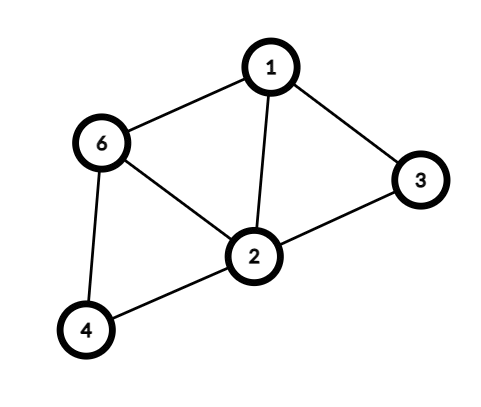
\includegraphics[width=0.36\textwidth]{3636.png}
        \end{center}
    \end{block}
    \begin{itemize}
        \item[$\rightarrow$] Đường đi \(3\to1\to6\to4\) là một đường đi đơn
        \item[$\rightarrow$] Đường đi \(3\to1\to2\to3\) là một ví dụ cho chu trình
        \item[$\rightarrow$] Còn ví dụ về đường đi có trọng số chúng ta sẽ nói rõ hơn vào phần sau
    \end{itemize}
\end{frame}


\section{PATH by DFS}
\begin{frame}{PATH by DFS}
    \begin{block}{}
        \begin{itemize}
            \item Như chúng ta đã biết, thuật toán DFS trong đồ thị cho phép duyệt và đi đến toàn bộ đỉnh của đồ thị 1 lần.
                  \pause
            \item Nhưng chỉ hàm DFS thông thường thì chúng ta chỉ có thể làm các bài đơn giản như check 1 đỉnh có thể đến được từ 1 đỉnh khác hay không. Nhưng trong chuyên đề này chúng ta cần nhiều hơn thế từ nó.
                  \pause
            \item Để có thể tìm được đường đi từ đỉnh u đến đỉnh v (giả sử) bằng DFS, chúng ta cần thêm 1 mảng par[], với par[i] là đỉnh cha của đỉnh i khi duyệt dfs từ đỉnh nguồn u
                  \pause
            \item Bên cạnh đó, nếu chỉ mỗi mảng par thì vẫn chưa đủ, chúng ta cần phải có 1 hàm trace để có thể lần lại đường đi đã được thực hiện bởi DFS
        \end{itemize}
    \end{block}
\end{frame}


\begin{frame}{PATH by DFS}
    \begin{alertblock}{Mã giả}
        \begin{center}
            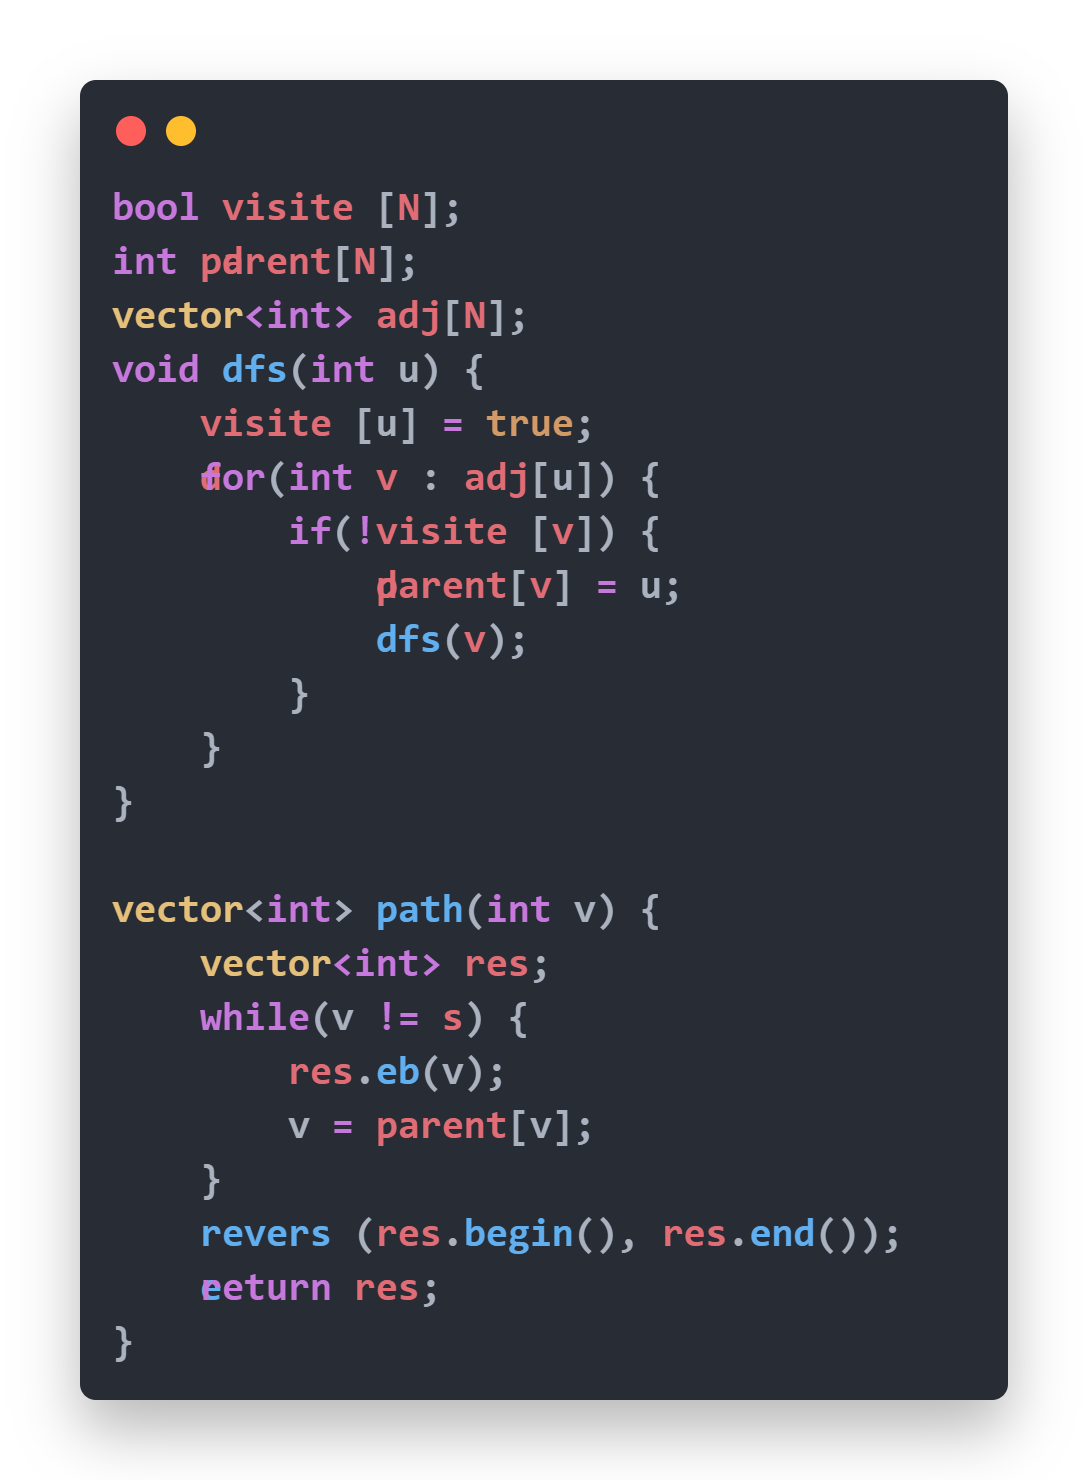
\includegraphics[width=0.415\textwidth]{codepathdfs.png}
        \end{center}
    \end{alertblock}
\end{frame}

\begin{frame}{PATH by DFS}
    \begin{block}{}
        \begin{itemize}
            \item[$\rightarrow$] Như chúng ta có thể nhận thấy từ mã giả, việc thăm được kiểm soát bởi mảng visited, vì vậy DFS sẽ lấy duy nhất 1 đường đi từ u đến v được duyệt trước mặc dù trong 1 đồ thị thì có thể có rất nhiều đường đi từ u đến v.
                  \pause
            \item[$\rightarrow$] Đường đi được trace lại phải lấy đảo ngược vì chúng ta đang đi ngược từ đỉnh đến đến đỉnh ban đầu
                  \pause
            \item[$\rightarrow$] Nếu muốn thì bạn có thể sort trước mảng danh sách kề, điều đó sẽ làm cho đường đi bạn lấy được là đường đi có thứ tự từ điển nhỏ nhất, còn nếu không, nó chỉ cho ra 1 đường đi bất kì phụ thuộc vào mảng danh sách kề của bạn hiện tại
        \end{itemize}
    \end{block}
\end{frame}


\section{PATH by BFS}
\begin{frame}{PATH by BFS}
    \begin{alertblock}{Khái quát}
        \begin{itemize}
            \item[$\rightarrow$] Nhìn chung, DFS và BFS không khác nhau trong việc nó chỉ duyệt qua tất cả các đỉnh có thể thăm từ 1 đỉnh bất kì, chúng khác nhau theo cách duyệt khi 1 cái là duyệt theo chiều sâu còn 1 cái là duyệt theo chiều rộng.
                  \pause
            \item[$\rightarrow$] Vì vậy, ở đây chúng ta vẫn cần ở BFS 1 mảng par và 1 hàm trace để có thể tìm được đường đi trên đồ thị bằng nó
                  \pause
            \item[$\rightarrow$] tương tự với DFS, code BFS trong vấn đề này không quá phức tạp khi cách trace và vis cũng tương tự như DFS, mã giả như sau:
        \end{itemize}
    \end{alertblock}
\end{frame}


\begin{frame}{PATH by BFS}
    \begin{alertblock}{Mã giả}
        \begin{center}
            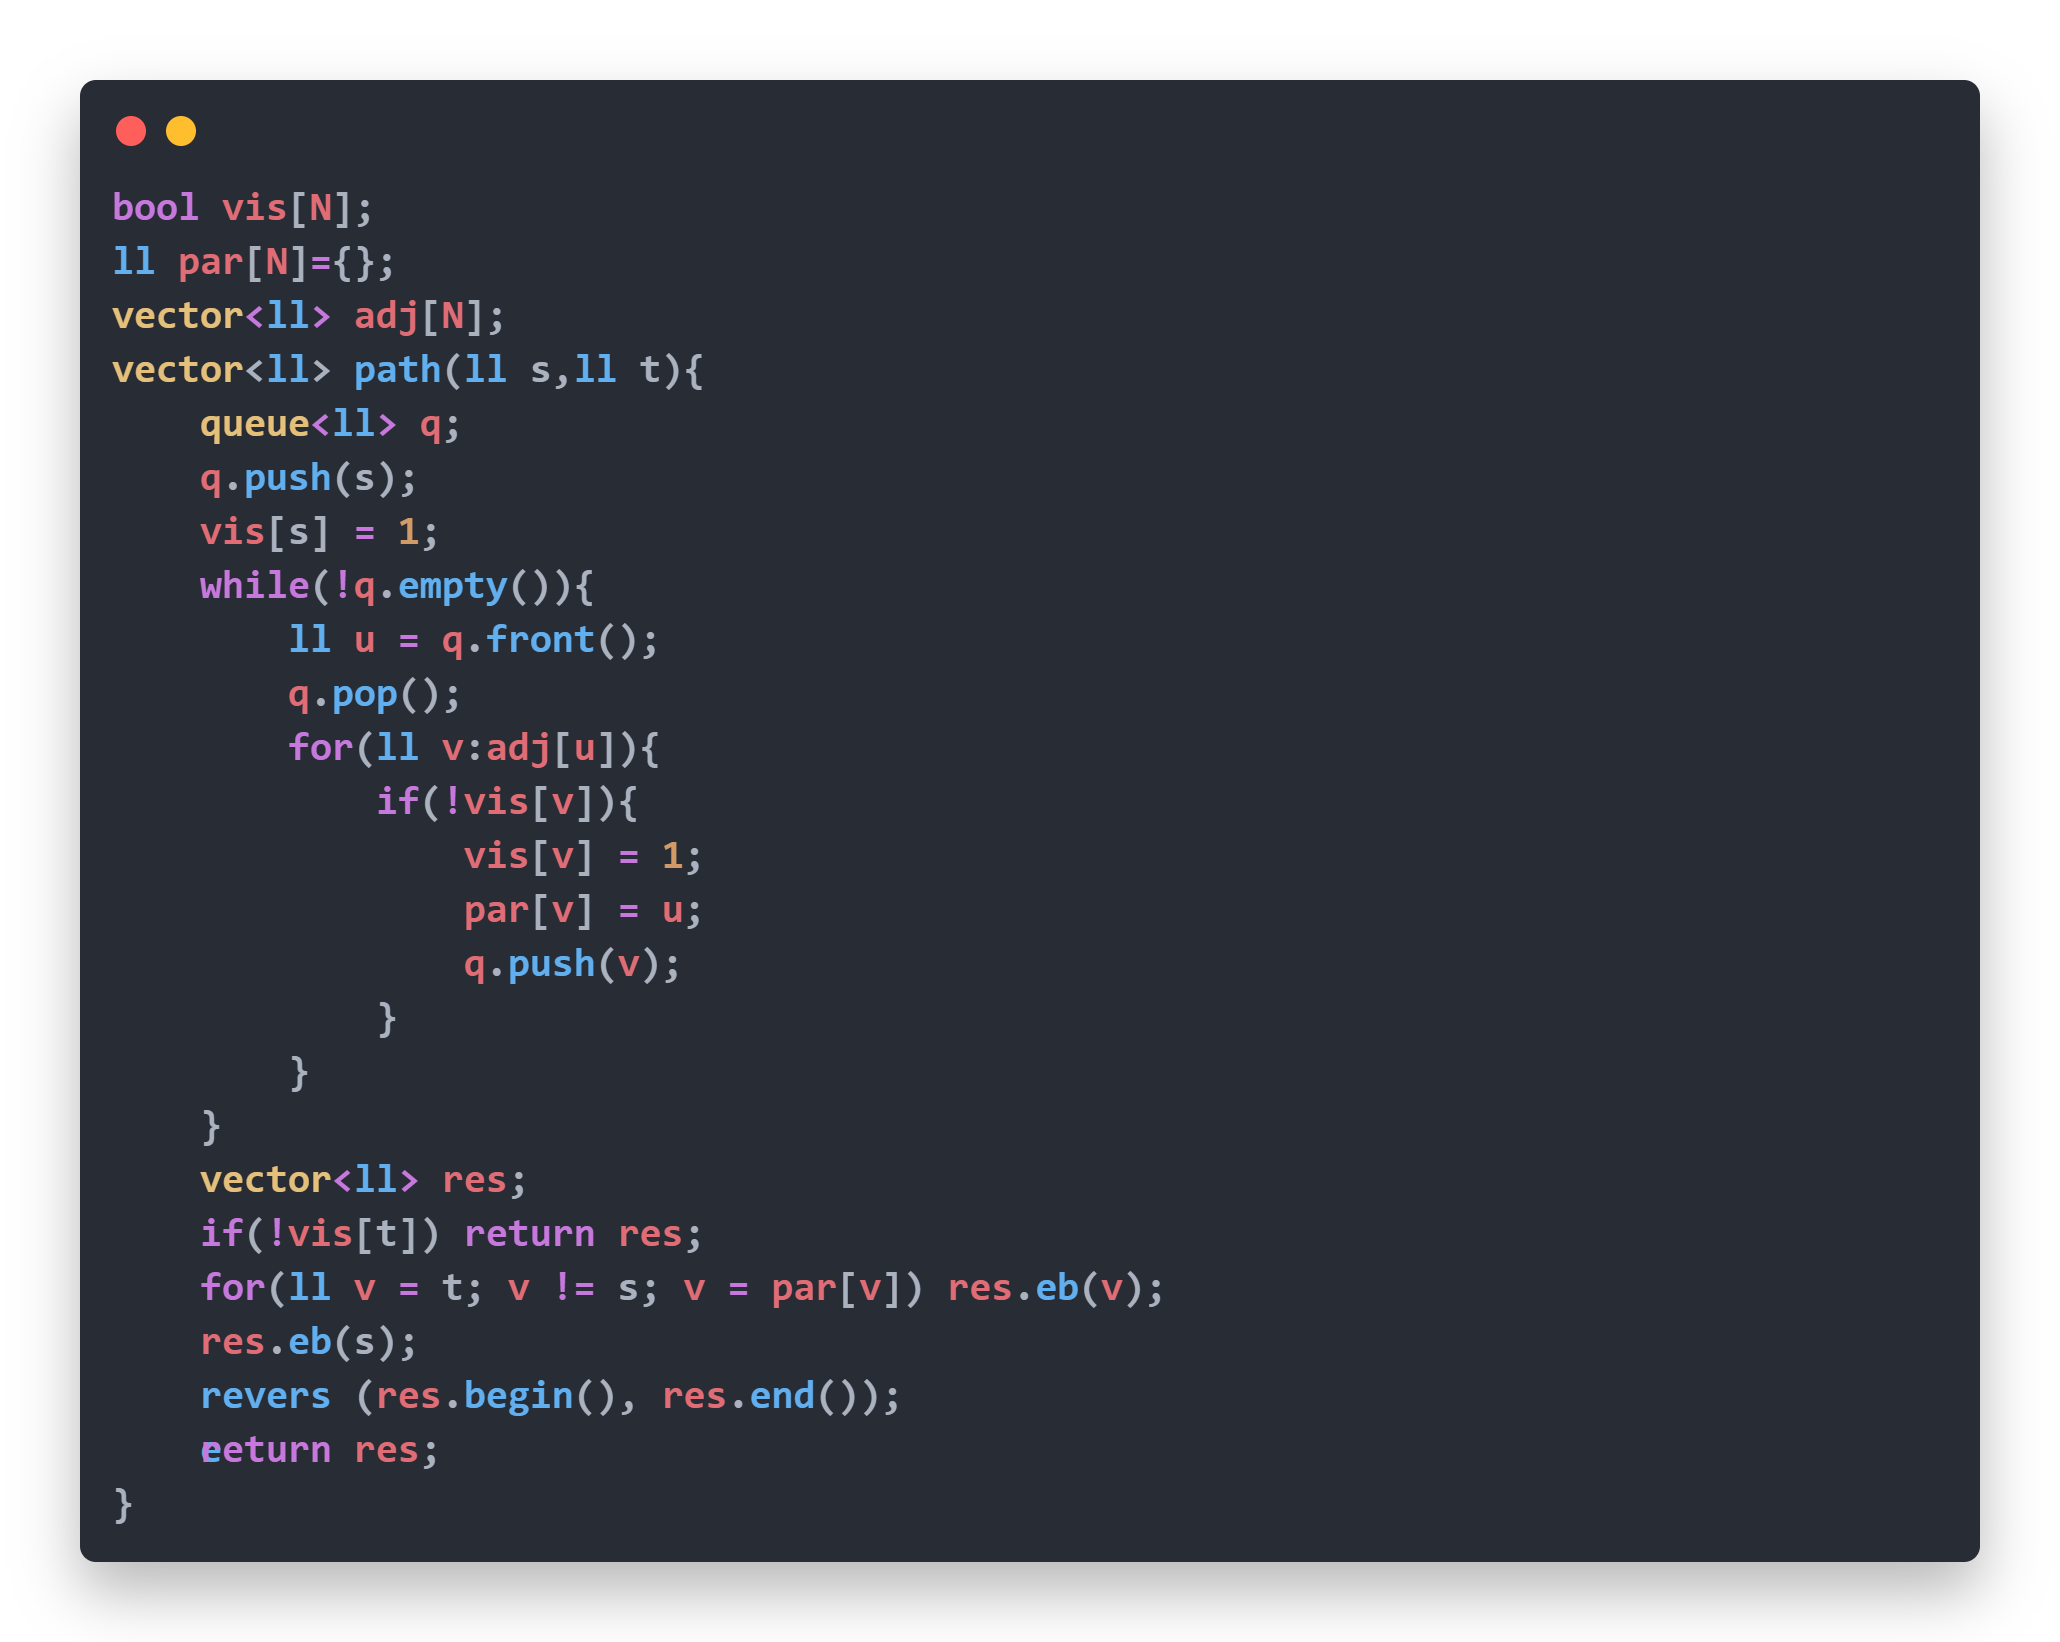
\includegraphics[width=0.7\textwidth]{codepathbfs.png}
        \end{center}
    \end{alertblock}
\end{frame}


\begin{frame}{PATH by BFS}
    \begin{exampleblock}{}
        \begin{itemize}
            \item [$\rightarrow$] Tương tự như DFS, đường đi được trace lại phải lấy đảo ngược vì chúng ta đang đi ngược từ đỉnh đến đến đỉnh ban đầu
                  \\
                  \pause
            \item [$\rightarrow$] Nếu muốn thì bạn có thể sort trước mảng danh sách kề, điều đó sẽ làm cho đường đi bạn lấy được là đường đi ngắn nhất có thể, còn nếu không, nó chỉ cho ra 1 đường đi bất kì phụ thuộc vào mảng danh sách kề của bạn hiện tại
                  \\
                  \pause
            \item [$\rightarrow$] Điểm khác biệt lớn nhất giữa DFS và BFS trong việc tìm đường đi đó là khi mảng danh sách kề được sort, nếu như DFS sẽ cho ra đường đi có thứ tự từ điển nhỏ nhất thì BFS sẽ luôn cho ra đường đi ngắn nhất có thể từ u đến v
        \end{itemize}
    \end{exampleblock}
\end{frame}




\section{Thuật Floyd-Warshall}

\begin{frame}{Floyd-Warshall}
    \begin{alertblock}{Khái quát}
        \begin{itemize}
            \item[$\rightarrow$] Floyd-Warshall là thuật toán tính \textbf{tất cả cặp đường đi ngắn nhất} trong đồ thị có trọng số (có thể âm, nhưng không có chu trình âm)
                  \pause
            \item[$\rightarrow$] Sử dụng cơ sở \textbf{dynamic programming(DP)}:
                  \(\text{dist}[i][j] = \text{chi phí đường đi ngắn nhất từ i đến j}\)
                  \pause
            \item[$\rightarrow$] Khác với DFS/BFS, Floyd-Warshall không dựa trên duyệt sâu hay rộng, mà cập nhật từ các đỉnh trung gian
        \end{itemize}
    \end{alertblock}
\end{frame}

\begin{frame}{Floyd-Warshall}
    \begin{alertblock}{Mã giả}
        \begin{center}
            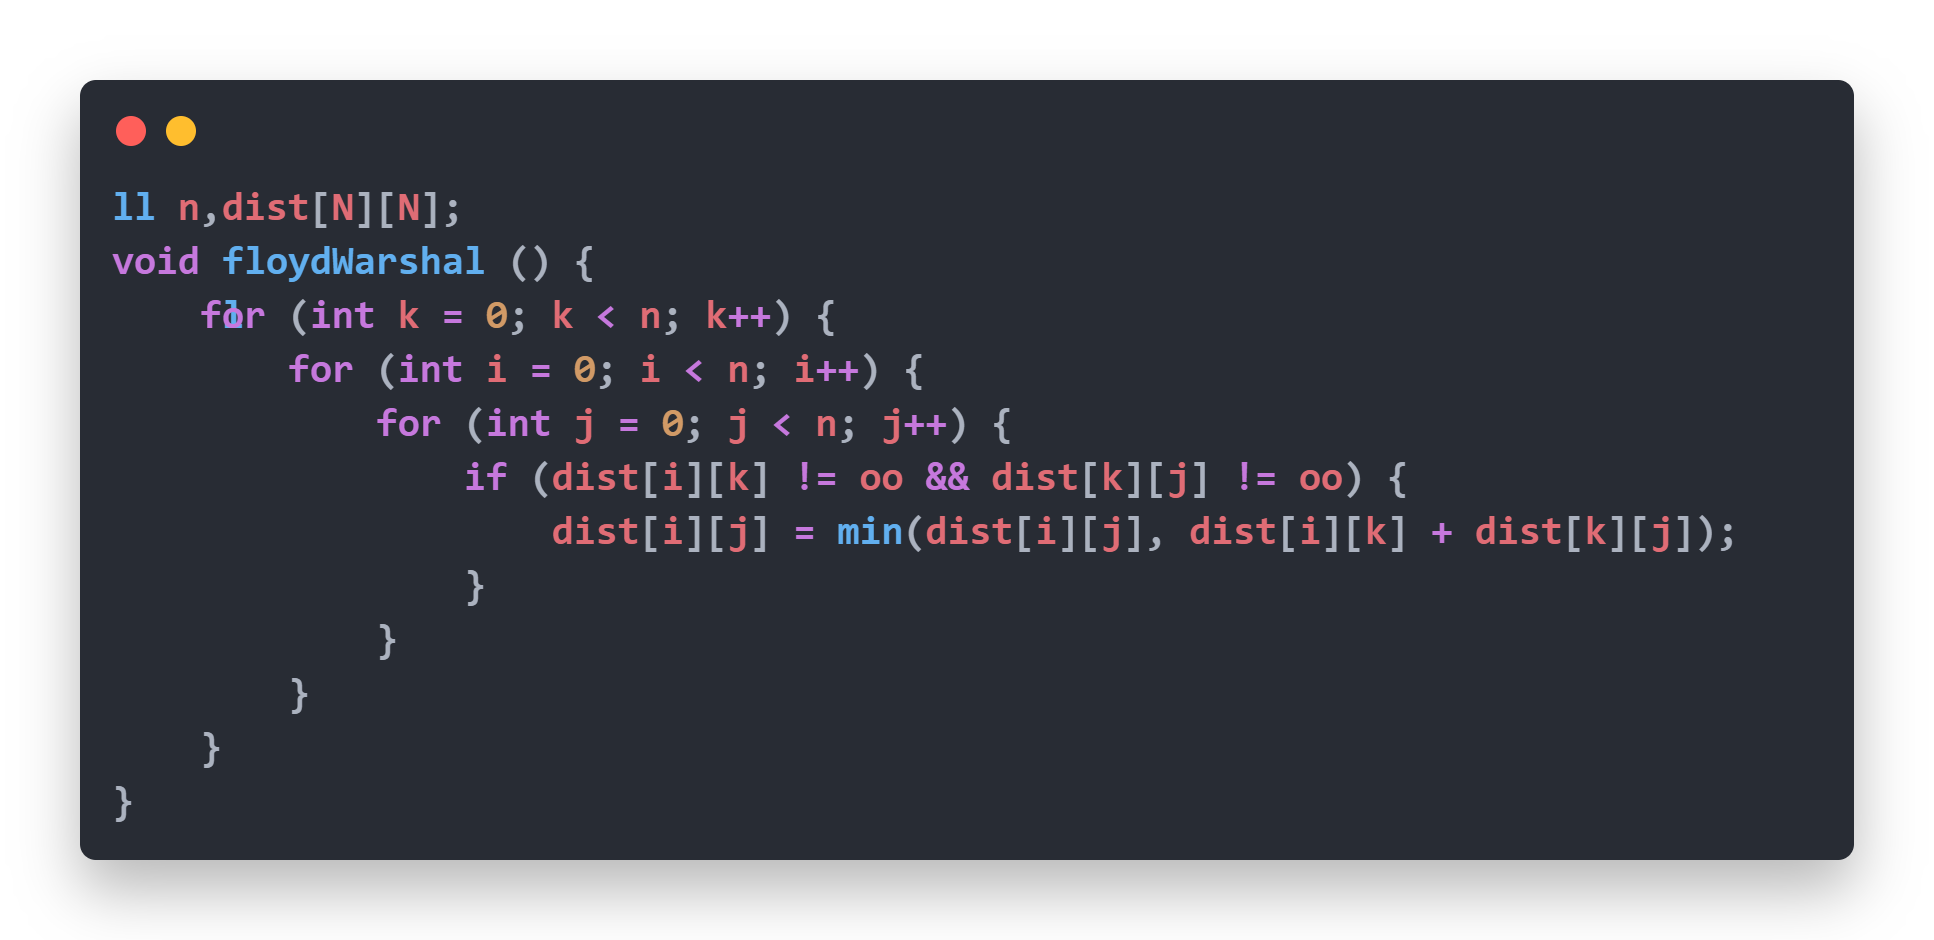
\includegraphics[width=0.7\textwidth]{floyd.png}
        \end{center}
    \end{alertblock}
\end{frame}

\begin{frame}{Floyd-Warshall}
    \begin{block}{}
        \begin{itemize}
            \item[$\rightarrow$] như vậy, ta có thể thấy rằng, floyd là một thuật toán khá đơn giản để tìm đường đi ngắn nhất giữa 2 đỉnh bất kì trong đồ thị với độ phức tạp khi lấy kết quả chỉ đơn giản là O(1) do dựa trên cách hoạt động của DP.
                  \pause
            \item[$\rightarrow$] Tuy nhiên, điểm yếu lớn nhất của thuật toán này đó là độ phức tạp O(\( n^3 \)) khi phải cập nhật tất cả cặp đường đi ngắn nhất trong đồ thị, điều này làm cho nó không phù hợp với các đồ thị lớn
                  \pause
            \item[$\rightarrow$] Để khắc phục điểm yếu này, chúng ta có thể sử dụng các thuật toán khác như Dijkstra hoặc Bellman-Ford để tìm đường đi ngắn nhất từ một đỉnh nguồn đến tất cả các đỉnh khác, sau đó lặp lại quá trình này cho mỗi đỉnh trong đồ thị để có được tất cả cặp đường đi ngắn nhất với độ phức tạp O(\( n \cdot (E + V \log V) \)) khi sử dụng Dijkstra với hàng đợi ưu tiên.
        \end{itemize}
    \end{block}
\end{frame}


\section{Thuật Dijkstra}

\begin{frame}{Dijkstra}
    \begin{alertblock}{Khái quát}
        \begin{itemize}
            \item[$\rightarrow$] Dijkstra là thuật toán tìm \textbf{đường đi ngắn nhất từ 1 nguồn} u đến tất cả các đỉnh còn lại trong đồ thị có trọng số không âm.
                  \pause
            \item[$\rightarrow$] Sử dụng cấu trúc \textbf{priority queue / heap} để luôn chọn đỉnh có khoảng cách ngắn nhất chưa được duyệt.
                  \pause
            \item[$\rightarrow$] Tương tự DFS/BFS, chúng ta cần mảng \textbf{dist[]} lưu khoảng cách ngắn nhất và mảng \textbf{par[]} để trace đường đi.
                  \pause
            \item[$\rightarrow$] Khi cập nhật đường đi: nếu đi qua nút u đến v mà dist[u] + w(u,v) < dist[v] thì cập nhật dist[v] và par[v] = u.
        \end{itemize}
    \end{alertblock}
\end{frame}

\begin{frame}{Dijkstra}
    \begin{alertblock}{Mã giả}
        \begin{center}
            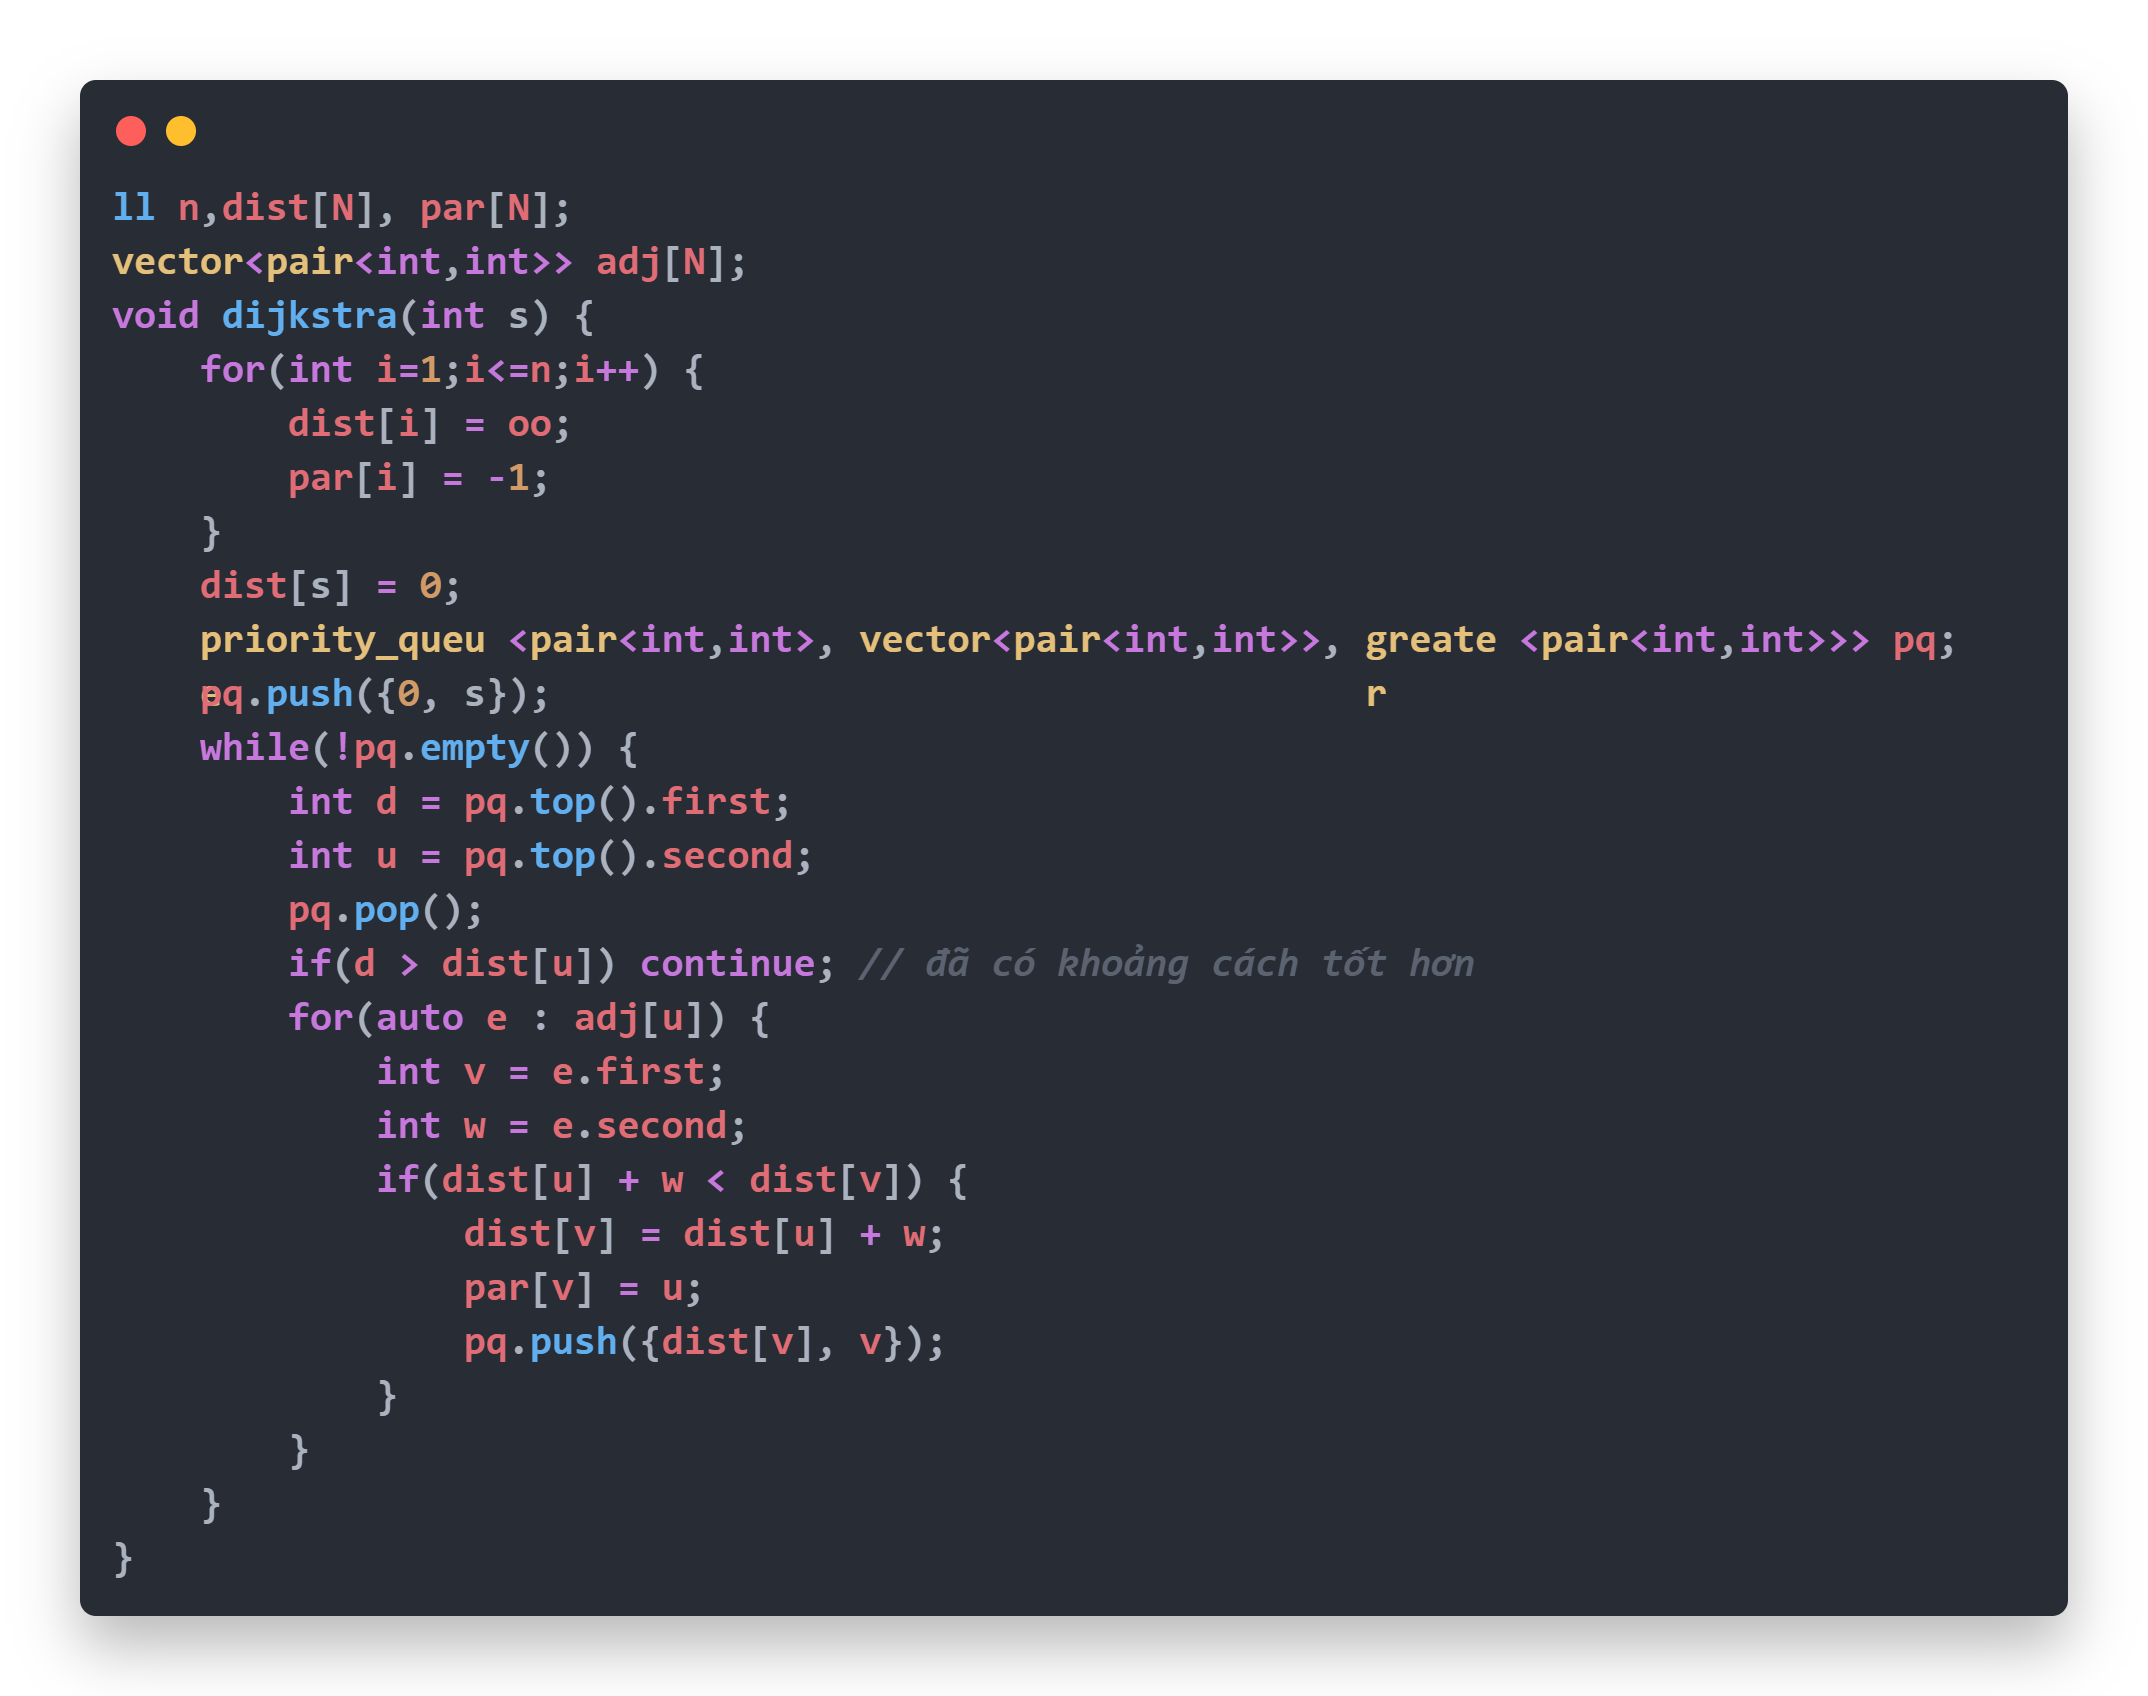
\includegraphics[width=0.72\textwidth]{dijktra.png}
        \end{center}
    \end{alertblock}
\end{frame}

\begin{frame}{Dijkstra}
    \begin{block}{Tổng quát}
        \begin{itemize}
            \item[$\rightarrow$] so với phương phát floyd, Dijkstra chỉ tập trung vào việc tìm đường đi ngắn nhất từ 1 nguồn đến tất cả các đỉnh còn lại, trong khi Floyd-Warshall tính tất cả cặp đường đi ngắn nhất.
                  \pause
            \item[$\rightarrow$] đánh đổi cho sự bất tiện khi chỉ có thể tìm đường đi ngắn nhất từ 1 nguồn, Dijkstra có độ phức tạp thấp hơn nhiều so với Floyd-Warshall, đặc biệt là trên các đồ thị thưa (sparse graphs).
                  \pause
            \item[$\rightarrow$] với độ phức tạp O((V + E) log V) khi sử dụng heap, Dijkstra thường được ưa chuộng trong các ứng dụng thực tế như định tuyến mạng, bản đồ, và các hệ thống GPS cũng như đây là một trong những thuật toán tuyệt vời nhất để tìm đường đi ngắn nhất trong đồ thị có trọng số không âm.

        \end{itemize}
    \end{block}
\end{frame}

\begin{frame}{Dijkstra - Lưu ý}
    \begin{exampleblock}{Điểm khác biệt với DFS/BFS}
        \begin{itemize}
            \item[$\rightarrow$] DFS: chỉ tìm 1 đường đi, không đảm bảo ngắn nhất về số bước hay trọng số.
            \item[$\rightarrow$] BFS: tìm đường đi ngắn nhất về số bước, nhưng chỉ áp dụng khi trọng số bằng 1.
            \item[$\rightarrow$] Dijkstra: tìm đường đi ngắn nhất theo trọng số >=0.
            \item[$\rightarrow$] Floyd-Warshall: tìm tất cả cặp đường đi ngắn nhất, dùng DP, độ phức tạp \(O(n^3)\).
        \end{itemize}
    \end{exampleblock}
\end{frame}



\section{Tổng kết}

% ===== END =====
\begin{frame}{Kết thúc}
    \centering
    \vspace{0.8cm}

    {\Huge \textbf{Cảm ơn thầy cô và các bạn đã theo dõi!}}

    \vspace{1cm}
    {\Large Xin chân thành cảm ơn}

    \vspace{1.2cm}

    \vfill

\end{frame}

\end{document}